\chapter{Role of precursors in growth of monolayer $WS_2$}

In this chapter the CVD growth of $WS_2$ using different precursors is investigated. The as grown samples were characterised by Raman and PL spectroscopy as well as XPS, XRD, AFM and electrical measurements. As a result it was concluded that using $H_2WO_4 + NaCl$ at 850 {\degree}C gives best results. Such grown samples exhibit biggest flakes up to 200 $\mu m$ in size as well as show the strongest and most narrow PL peak with 36 meV FWHM. The samples grown using $H_2WO_4 + NaCl$ at 950 {\degree}C show also best transistor electron mobility in monolayer CVD grown $WS_2$ while that grown using $WO_3 + NaCl$ at 950 {\degree}C shows best transistor electron mobility in bilayer CVD grown $WS_2$. 

\section{Introduction}
	
Monolayers of transition metal sulphides and selenides exhibit range of interesting properties such as strong light absorption in the IR and visible range \cite{AtomicallyThinMoS2ANewDirect-GapSemiconductor}\cite{ExtraordinarySunlightAbsorptionAndOneNanometerThickPhotovoltaicsUsingTwo-DimensionalMonolayerMaterials}\cite{EvolutionOfElectronicStructureInAtomicallyThinSheetsOfWS2AndWSe2}, valley polarisation \cite{ControlOfValleyPolarizationInMonolayerMoS2ByOpticalHelicity} \cite{ValleyPolarizationInMoS2MonolayersByOpticalPumping}, spin-orbit interactions \cite{CoupledSpinAndValleyPhysicsInMonolayersOfMoS2AndOtherGroup-VIDichalcogenides}\cite{GiantSpin-orbit-inducedSpinSplittingInTwo-dimensionalTransition-metalDichalcogenideSemiconductors}, tightly bound excitons \cite{TightlyBoundTrionsInMonolayer} or second-harmonic generation \cite{ProbingSymmetryPropertiesOfFew-LayerMoS2Andh-BNByOpticalSecond-HarmonicGeneration}. Some of these effects can be attributed to the lack of free dangling bonds and configuration of d-orbitals \cite{TheTransitionMetalDichalcogenidesDiscussionAndInterpretationOfTheObservedOpticalElectricalAndStructuralProperties}, \cite{ElectronicPropertiesOfMoS2Nanoparticles}.

Among these materials one of the most promising is the $WS_2$. Its visible range bandgap of 2eV as well as an easy and safe manufacturing route via CVD makes it one of the more interesting and studied TMDCs. The typical characterisation by photoluminescence spectroscopy allows to probe the varying synthesis conditions, the grain boundaries or defect population \cite{ExtraordinaryRoomTemperaturePhotoluminescenceInTriangularWS2Monolayers} \cite{doi:10.1021/nn4046002} \cite{Li2015} \cite{Rong2014}. The PL efficiency in as-grown monolayer $WS_2$ produced via CVD growth shows {$\sim$}2-6\% efficiency \cite{doi:10.1021/nn4046002}\cite{Yuan2015} \cite{doi:10.1021/nn403682r}. This efficiency is caused mostly by defect-mediated non-radiative recombination centres \cite{Amani2015}. LEDs have been successfully produced \cite{doi:10.1021/nl500171v} showing external quantum efficiency up to 10\% \cite{Zeng2016}\cite{Withers2015}. $WS_2$ is typically a n-type semiconductor due to the presence of sulphur vacancies \cite{ExtraordinaryRoomTemperaturePhotoluminescenceInTriangularWS2Monolayers}\cite{doi:10.1021/nn5059908}\cite{Iqbal2015}. In order to utilise this material in any potential future applications a reliable and scalable manufacturing method must be developed to ensure a high quality crystal on the wafer scale area. The main method for $WS_2$ synthesis that satisfies these conditions is Chemical Vapour Deposition (CVD) \cite{Hofmann1988}. The growth of tungsten based TMDCs have been less successful than the equivalent molybdenum based TMDCs and has produced mostly isolated flakes of up to 40 $\mu m$ \cite{ExtraordinaryRoomTemperaturePhotoluminescenceInTriangularWS2Monolayers} \cite{doi:10.1021/nn403454e} \cite{Rong2014} \cite{doi:10.1021/nn400971k}\cite{doi:10.1021/acsnano.5b01480}\cite{Fu2015}\cite{Lee2013}. Even larger films of monolayer $WS_2$ have been shown, however they also exhibit low carrier mobility \cite{Kang2015}\cite{Gao2015}. In the typical CVD synthesis process the sulphur and tungsten oxide are evaporated simultaneously in a tubular furnace with a constant flow of carrier gas like argon at temperatures of at least 900 {\degree}C \cite{ExtraordinaryRoomTemperaturePhotoluminescenceInTriangularWS2Monolayers}\cite{doi:10.1021/nn403454e}\cite{Rong2014}\cite{doi:10.1021/nn400971k}\cite{doi:10.1021/acsnano.5b01480}\cite{Fu2015}\cite{Lee2013}. Such growth is predicated by topotacic transformation leading to low density distribution of domains on an amorphous \cite{ExtraordinaryRoomTemperaturePhotoluminescenceInTriangularWS2Monolayers}\cite{doi:10.1021/nn403454e}\cite{doi:10.1021/nn400971k}\cite{Fu2015}\cite{Lee2013} or crystalline substrate \cite{Rong2014}\cite{doi:10.1021/acsnano.5b01480}\cite{doi:10.1021/nn503093k} possibly due to low evaporation rates of $WO_3$. Since $WO_3$ requires high temperatures of 950-1000 {\degree}C to evaporate while the $S$ becomes volatile at 90 {\degree}C the thermodynamics of the process are difficult to control. The low growth dictated by fast evaporation of $S$ leads to limited domain growth and lack of continuous layer. One of the proposed solutions have been to spread the $WO_3$ on the target substrate \cite{doi:10.1021/nn4046002}\cite{Li2015}\cite{Gao2015}\cite{Cong2013}\cite{Yun2015}\cite{Gong2015}\cite{Gong2014}. This has however led to low reproducibility, poor control of thickness and stoichiometry and unreacted material left on the substrate. Another approach has been to use more volatile $W$ precursors such as $WCl_6$\cite{Carmalt2003} or $W(CO)_6$\cite{Kang2015}\cite{Eichfeld2015} together with organic compounds as $S$ precursors. Such method while producing a large area domains at lower temperature has led to lower crystal quality and purity.

Here we propose a different method of CVD synthesis that allows for much larger flake growth of up to 800 $\mu m$ at temperature of 750 {degree}C. Such grown material exhibits high electron mobility in one and two layers of $WS_2$, higher than other values reported in literature. The photoluminescence peak is also very narrow at 36 meV FWHM at room temperature. 

\section{Results}
	
For the purpose of comparing the CVD synthesis method conditions the several sets of precursors were used: $WO_3$, $WO_3$ + NaCl and $H_2WO_4$ + NaCl. The standard growth procedure involves two separate crucibles placed at distance from each other in a quartz tube. Each of these crucibles is independently heated to ensure that the S and the W precursors evaporation rate is maximised at the same time. The vapours then are deposited on $SiO_2/Si$ (285 nm) substrate which is placed close to the W precursor crucible. The entire process is performed under low vacuum and a supply of Ar gas. The furnace setup can be seen in Figure \ref{fig:PaperSIFurnace}.

\begin{figure}[h]
	\begin{center}
		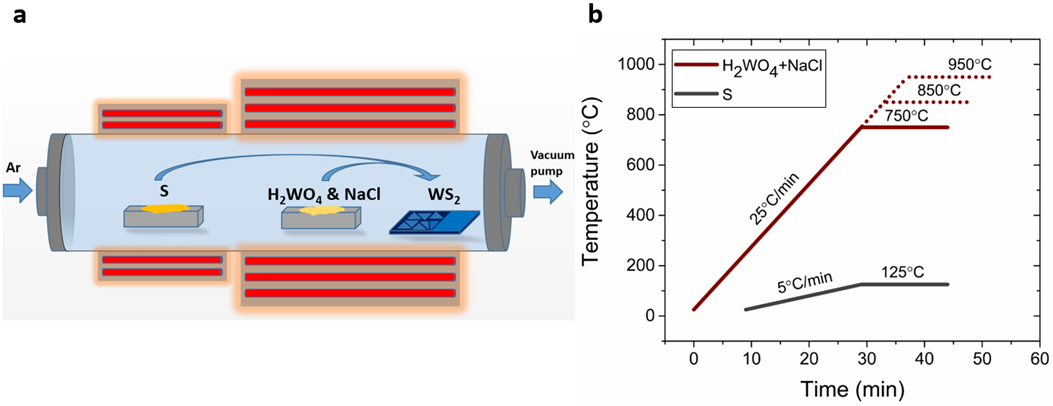
\includegraphics[scale=0.3]{PaperSIFurnace.png}
		\caption{Illustration of: (a) CVD tubular furnace set-up; (b) temperature profile of the sulphur and the W-precursors heaters respectively. The sulphur reaches 125 {\degree}C when the metal precursors are at the maximum temperature. The SiO2/Si wafers used as substrate for WS2 growth are placed 1-8 cm downstream the W-precursors crucible and they are subjected to the same temperature.}
		\label{fig:PaperSIFurnace}
	\end{center}
\end{figure} By following this method a reproducible deposition of large area flakes can be shown. As seen in Figure \ref{fig:PaperOptical} the size of the flakes increases from left to right as the precursors used ($WO_3$, $WO_3-NaCl$ and $H_2WO_4-NaCl$) change as well as demonstrating the lower temperature required to achieve these growths. All of these growths result in formation of triangular flakes with sharp edges and uniformity of colour throughout which suggest a high quality, pristine material across the flake. 
The growth using only $WO_3$ results in formation of small flakes of 10 $\mu m$ at 950 {\degree}C while no growth occurs at lower temperatures (Figure \ref{fig:PaperOptical}. This can be explained by the high sublimation temperature of $WO_3$.

\begin{figure}[h]
\begin{center}
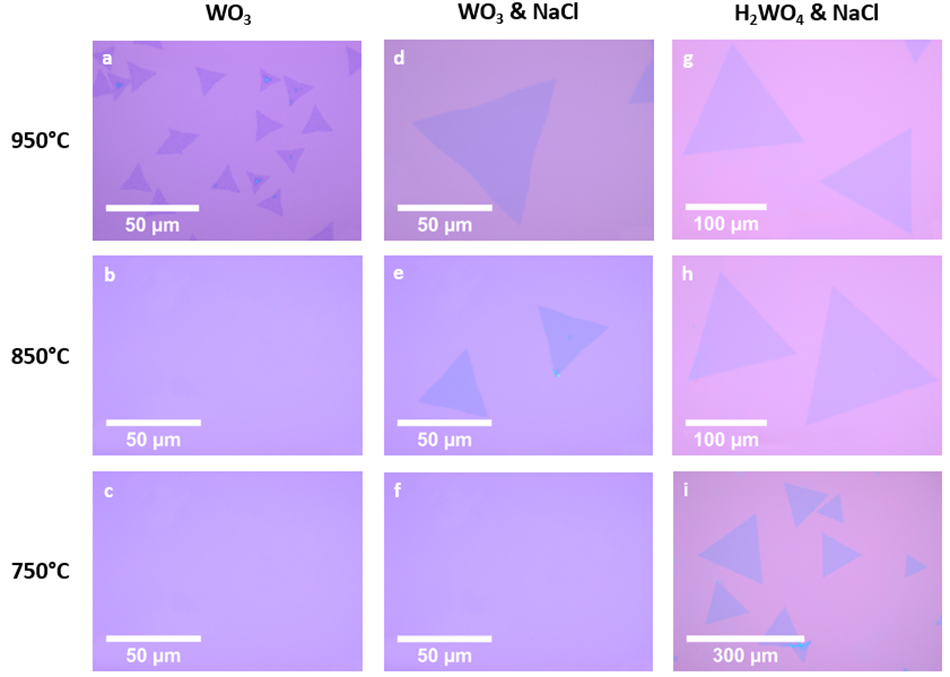
\includegraphics[scale=0.3]{PaperOptical.png}
\caption{Optical micrographs of $WS_2$ triangles grown on $SiO_2/Si$ substrates at different temperatures and using different precursors: (a) $WO_3$ at  950 {\degree}C; (b) $WO_3$ at 850 {\degree}C; (c) $WO_3$ at 750 {\degree}C; (d) $WO_3 + NaCl$ at 950 {\degree}C; (e) $WO_3+NaCl$ at 850 {\degree}C; (f) $WO3 + NaCl$ at 750 {\degree}C, the OM appears as a bare SiO2 substrate; (g) $H_2WO_4 + NaCl$ at 950 {\degree}C; (h) $H_2WO_4 + NaCl$ at 850 {\degree}C; (i) $H_2WO_4 + NaCl$ at 750 {\degree}C.}
\label{fig:PaperOptical}
\end{center}
\end{figure}

The growth can also be observed using $WO_3 + NaCl$ at 950 {\degree}C and 850 {\degree}C with the former showing flakes of size of about 60 $\mu m$ while the latter showing smaller flakes of about 30 $\mu m$ in size. To explain this difference in size a Robinson \& Robin model can be used which states that at higher temperatures the diffusivity of the adsorbed precursors is favourable to the expansion of the existing domains. On the other hand the desorption of the adsorbed species is high leading which limits the supersaturation and formation of new domains. If the temperature is lowered even further to 750 {\degree}C then no growth is observed at all, most likely due to slow evaporation of $WO_3$ precursor. 

With the change of precursors from $WO_3$ to $H_2WO_4$ a signifacnt change in size of flakes is observed at 850 {\degree}C  and higher temperatures with lengths exceeding 200 $\mu m$. Additionally the growth have been shown to occur at 750 {\degree}C with flakes of the size of 50-200 $\mu m$. Moreover continuous monolayer areas of up to 0.8 mm in size has been shown (Figure \ref{fig:PaperSIOpticalContinous}). By increasing the growth pressure (1.6 mbar to 13 mbar) at 950 {\degree}C bilayer $WS_2$ flakes can be preferentially formed (Figure \ref{fig:PaperSIOpticalAFM}.

\begin{figure}[h]
	\begin{center}
		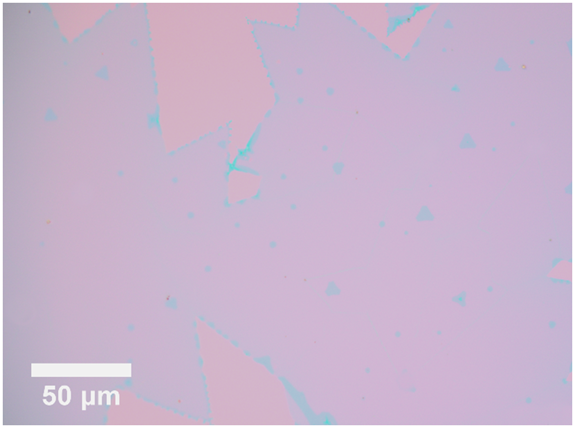
\includegraphics[scale=0.3]{PaperSIOpticalContinous.png}
		\caption{Optical micrograph of continuous layer of $WS_2$}
		\label{fig:PaperSIOpticalContinous}
	\end{center}
\end{figure}

\begin{figure}[h]
	\begin{center}
		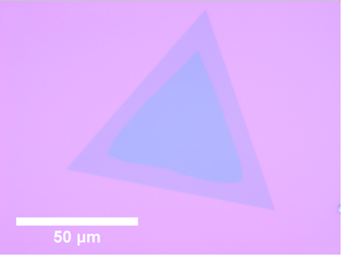
\includegraphics[scale=0.3]{PaperSIOpticalAFM.png}
		\caption{Optical micrograph of $WS_2$ bilayer}
		\label{fig:PaperSIOpticalAFM}
	\end{center}
\end{figure}

%\todo[inline]{Original paper starts here. To be replaced or rewritten}

By replacing WO3 with H2WO4 the lateral size of the WS2 monolayered domains significantly increases (Figure 1g,h,i). The triangular crystals have edge lengths exceeding 200 {$\mu$}m at temperatures higher than 850 {\degree}C and between 50-200 {$\mu$}m at 750 {\degree}C (Figure 1g,h,i). Continuous polycrystalline monolayer coverage has been obtained over areas of {$\sim$}0.8 mm extension (Figure S2). Increasing the growth pressure (from 1.6 mbar to 13 mbar) at 950 {\degree}C bilayered WS2 flakes are preferentially formed (Figure S3). To understand the facilitated synthesis of WS2 using H2WO4 and NaCl, we conducted X-ray diffraction (XRD) analysis of the reaction products between H2WO4+NaCl and WO3+NaCl systems at different temperatures (500 {\degree}C, 650 {\degree}C and 750 {\degree}C) to understand the chemical differences (Figure S4). We found that the main products of the reactions between NaCl and H2WO4 are: NaxWyOz and tungsten oxychloride (WClO4 and WO2Cl2). The NaxWyOz possesses a high evaporation temperature as it remains in the crucible (Figure S5) after the synthesis of WS2 is completed. Further, using this compound as precursors for a new growth of WS2 at 950 {\degree}C did not lead to the formation of any WS2 flakes, confirming the high evaporation temperature. On the bases of previous studies on the synthesis of bulk crystals, the formation of tungsten oxychloride species (WO2Cl2 and/or WOCl4) is likely to occur while the formation of metal halides is less favourable (e.g. WCl6) [ ][ ]. Tungsten oxychlorides are volatile already at 200 {\degree}C [ ] and they can be sulfidized in vapour phase and then be deposited onto the target substrate as atomic clusters. WOCl4 has been previously used [43] as precursor for the CVD synthesis of WS2 bulk films. Despite its strong tungsten oxygen double bonds, WOCl4 proved to be an effective precursor with a clean decomposition pathway in the CVD process without formation of tungsten oxysulfide. We have verified that using this precursor is indeed possible to obtain WS2 at temperatures as low as 550 {\degree}C (Figure S6a). The key role played by the oxyhalide species it becomes apparent if we try to grow WS2 by using only hydrated tungsten oxide. As this decomposes to form WO3, only small WS2 domains are observed with similar PL characteristics to the WO3 precursors-growth (Figure S6b). Furthermore, to confirm the key role played by Cl, we replaced NaCl with KCl and we obtained comparable growth results (Figure S6c).

% paper break

\begin{figure}[h]
	\begin{center}
		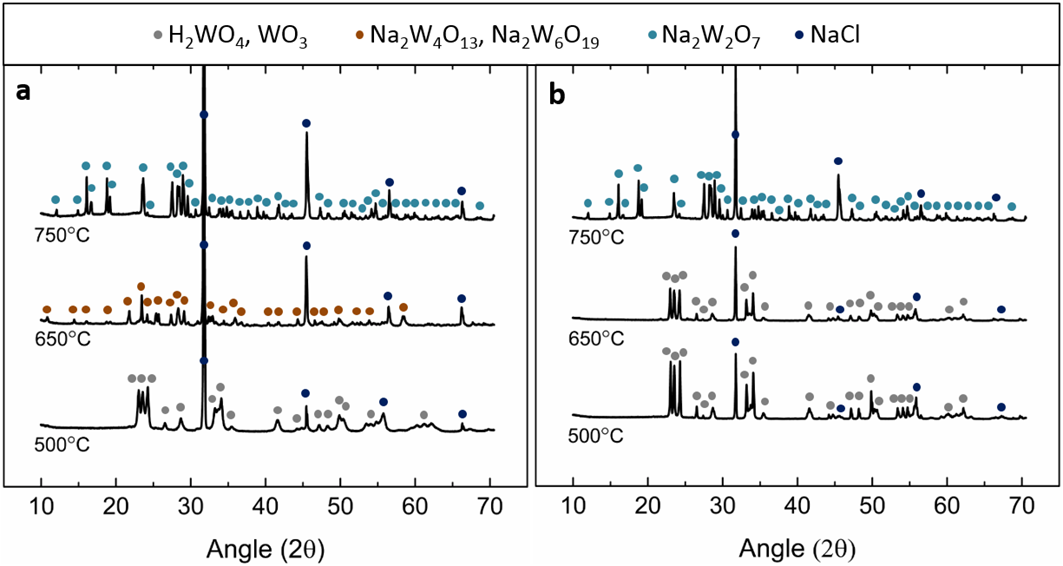
\includegraphics[scale=0.3]{PaperSIXRD.png}
		\caption{XRD pattern of the residual powder of W-precursors after thermal treatment at 500 {\degree}C, 650 {\degree}C and 750 {\degree}C respectivley, using (a) $H_2WO_4+NaCl$ and (b) $WO_3+NaCl$ as precursor.}
		\label{fig:PaperSIXRD}
	\end{center}
\end{figure}

\begin{figure}[h]
		\begin{center}
		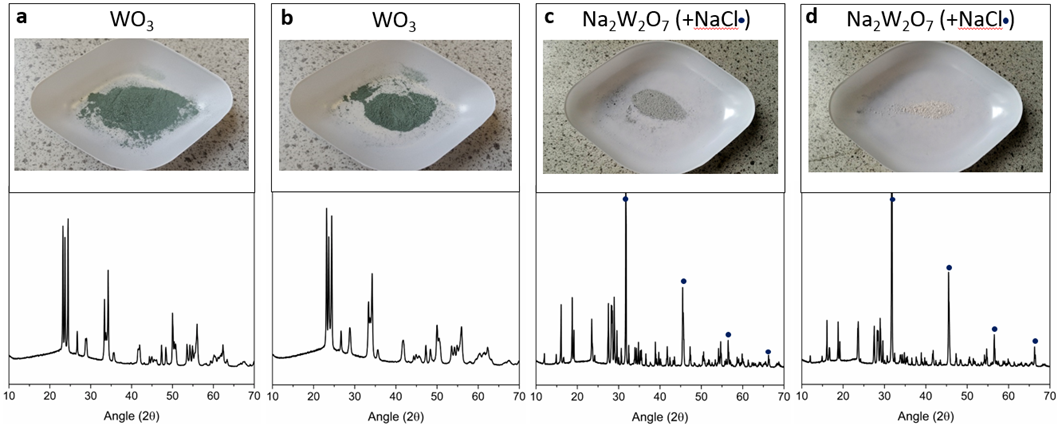
\includegraphics[scale=0.3]{PaperSIXRDOptical.png}
		\caption{Residual powders of the W-precursors and their XRD patterns after thermal treatment at 750{\degree}C using (a) $WO_3$, (b) $H_2WO_4$, (c) $WO_3+NaCl$, and (d) $H_2WO_4+NaCl$ as precursor. The blue dots in the XRD patterns indicate the presence of residual NaCl.}
		\label{fig:PaperSIXRDOptical}
	\end{center}
\end{figure}

The flakes were investigated using HRTEM to confirm high crystallinity of the material (Figure \ref{fig:PaperAFM}. The lattice constant measured in this way has been found to be 0.3 nm, which is consistent with that of 2H-WS2 (0.318 nm). The AFM characterisation allowed to confirm the presence of monolayer (Figure \ref{fig:PaperAFM}) and bilayer (Figure \ref{fig:PaperSIOpticalAFM} flakes with the step of 0.8 nm \cite{Wu2014}\cite{Rasmussen2015}.

The Raman spectroscopy characterisation of $WS_2$ flakes obtained under different growth conditions can be seen in Figure \ref{fig:PaperAFM}. All of these spectra exhibit the main 2 peaks at {$\sim$}(351{$\pm$}0.53) $cm^{−1}$ and {$\sim$}(417.6{$\pm$}1) $cm^{−1}$. The latter peak corresponds to the $A_{1g}$ vibrational mode while the former peak can be further resolved into two peaks, one related to 2LA vibrational mode and the second to $E^1_{2g}$. As seen in the Figure \ref{fig:PaperSIMapsIntensityE} and Figure \ref{fig:PaperSIMapsIntensityA} the distribution of intensity of both main peaks is uniform across the flakes. Similarly the difference between peak positions of $A_{1g}$ and $E^1_{2g}$ is also uniformly distributed as seen in Figure \ref{fig:PaperSIMapsDifference} and is equal to {$\sim$}(66.5{$\pm$}0.53) $cm^{−1}$ which is indicative of monolayer \cite{Withers2014}.

\begin{figure}[h]
\begin{center}
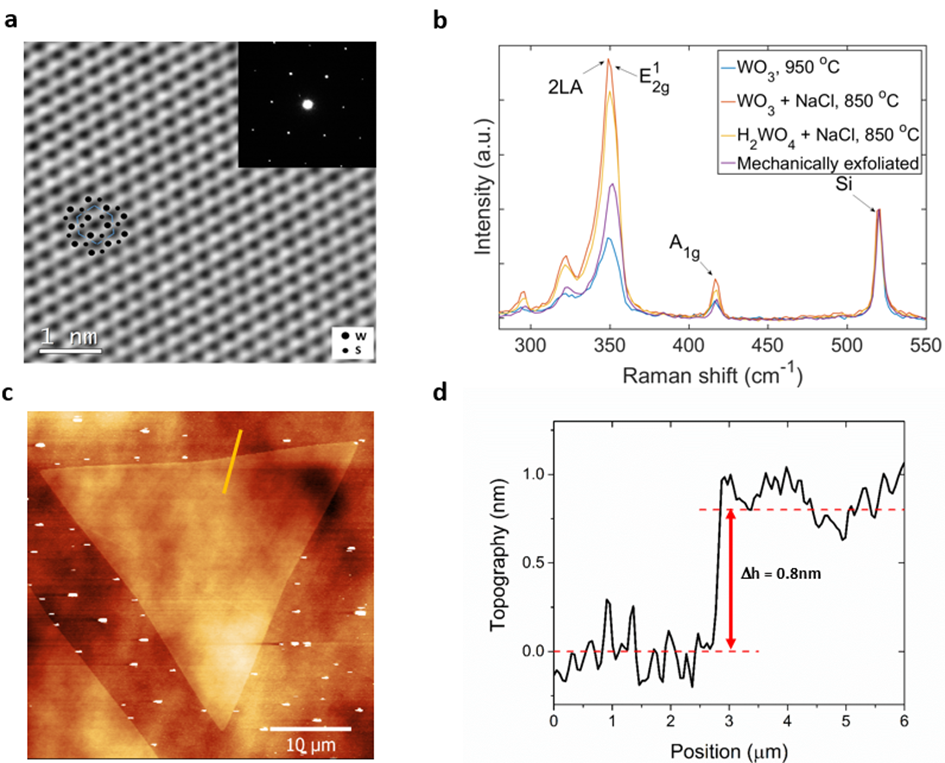
\includegraphics[scale=0.3]{PaperAFM.png}
\caption{Structural and physical characterization of WS2 triangles: (a) HRTEM image of the $WS_2$ lattice grown using $H_2WO_4+NaCl$, the inset report a selected diffraction area which show a hexagonal pattern. (b) Raman spectra showing the characteristics active modes of WS2 grown under different conditions and compared with mechanically exfoliated flakes. (c) AFM image and (d) corresponding thickness profile of monolayer $WS_2$.}
\label{fig:PaperAFM}
\end{center}
\end{figure}

As seen in Figure \ref{fig:PaperPLMaps} maps of PL intensity has been collected for samples grown using different growth condition. The sample grown using $WO_3$ at 950 {\degree}C appears to be trisected into 3 symmetrical areas. The intensity is lowest along the the trisecting lines and highest in the centre of each of the sub-triangles. The PL peak position is inversely proportional to the intensity of the PL peak as seen in Figure \ref{fig:PaperSIMapsPositionPL}. The distribution of the PL peak positions seems to be bimodal with maxima at 1.96 eV and 1.94 eV. The FWHM is distributed mostly uniformly with few small areas of greater and few of smaller FWHM (Figure \ref{fig:PaperSIMapsWidthPL} with the average value of 65 meV. These peak position and FWHM values are comparable with those reported in literature \cite{ExtraordinaryRoomTemperaturePhotoluminescenceInTriangularWS2Monolayers}\cite{Rong2014}\cite{Hu2016}\cite{Kang2015a}. The PL spectra taken from one of the three smaller parts of the flake are redshiftted by about 0.02 eV and are wider than average. This can be explained by the presence of defects, in particular sulfur vacancies, which effectively cause the $WS_2$ to be n-doped \cite{Hui2013}\cite{Peimyoo2014}. This in turn increases the trion population which introduces new peak, redshifted by about 30 meV, which results in overall shift and broadening of the PL peak \cite{Tongay2013}\cite{ExtraordinaryRoomTemperaturePhotoluminescenceInTriangularWS2Monolayers}. Additionally such localised changes in PL peak intensity and position can be caused by local strain \cite{Liu2014}\cite{Hui2013}. To investigate the potential effect of strain on the observed PL pattern a flake was cut using high power 532nm laser. As seen in Figure \ref{fig:PaperSIMapsCutting} the resulting pattern remains the same as before treatment. Therefore the observed pattern is most likely caused by the local variation in defect density \cite{Liu2016}.

By introducing the NaCl and mixing it with $WO_3$ precursor $WS_2$ samples are grown that exhibit higher energy and narrower PL peaks. The spectra are asymetric and can be therefore deconvoluted to obtain an exciton and trion component (Figure \ref{fig:PaperPLSpectraHistograms}). The spatial distribution of the PL position and width is mostly uniform throughout the flake. However the distribution of PL peak positions and FWHM across different flakes grown at the same conditions is bimodal (Figure \ref{fig:PaperPLSpectraHistograms}. The PL peak position is found to be ({$\sim$}1.95{$\pm$}0.002 eV and 1.96{$\pm$}0.002 eV) while the FWHM is ({$\sim$}43{$\pm$}2.8 meV and 51{$\pm$}3 meV) which is smaller than most reported works \cite{ExtraordinaryRoomTemperaturePhotoluminescenceInTriangularWS2Monolayers}\cite{Rong2014}\cite{Hu2016}\cite{Kang2015a}. This can be explained by smaller trion component in the PL spectrum which in turn means that $WS_2$ samples grown at these conditions contain less structural defects compared to the pure $WO_3$ growth. A difference in growth mechanism (topotactic or molecular conversion) which results in different defect distribution can be attributed to the differences in samples.

\begin{figure}[h]
\begin{center}
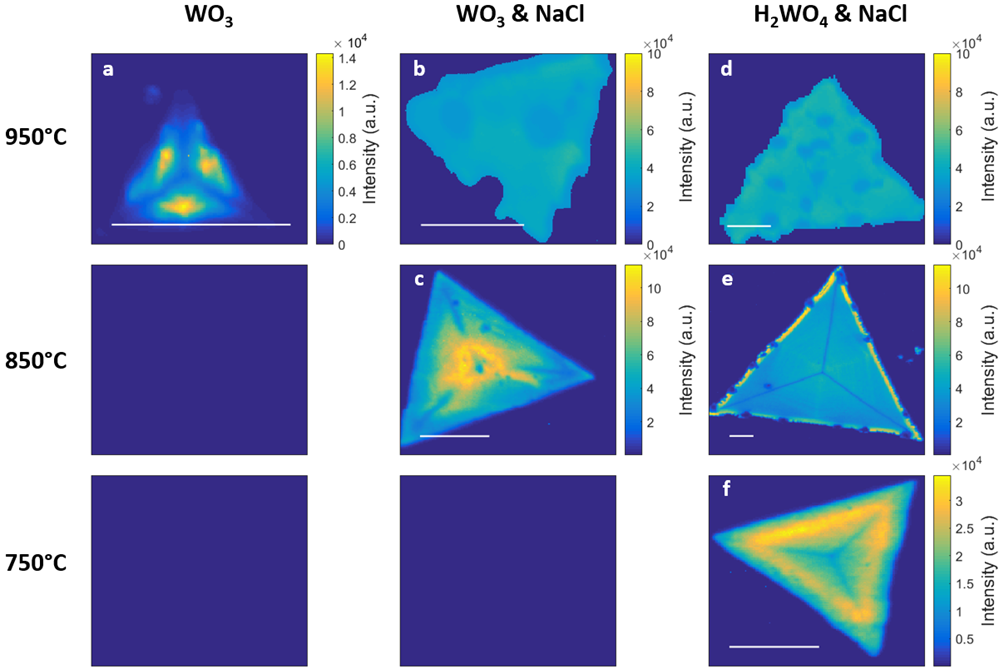
\includegraphics[scale=0.3]{PaperPLMaps.png}
\caption{Spatial maps of PL intensity of $WS_2$ grown in the conditions exemplified in Figure 1. The scale bar length is 10$\mu$m.}
\label{fig:PaperPLMaps}
\end{center}
\end{figure}

By changing the $WO_3$ precursor to the $H_2WO_4$ precursor a further shift in PL peak position, as well as increase in PL intensity and narrowing of he PL peak is observed as seen in Figure \ref{fig:PaperPLMaps}, \ref{fig:PaperPLSpectraHistograms}. The PL peak position distribution across the flake is narrow and is ({$\sim$}1.980{$\pm$}0.005 eV) which is higher than that of the $WO_3$ and $WO_3 + NaCl$ systems. The FWHM is found to be ({$\sim$}36{$\pm$}3 meV) which is also smaller than that of the $WO_3$ and $WO_3 + NaCl$ systems. The PL peak width is also smaller than that reported in literature for CVD grown \cite{ExtraordinaryRoomTemperaturePhotoluminescenceInTriangularWS2Monolayers}\cite{Rong2014}\cite{Hu2016}\cite{Kang2015a} exfoliated $WS_2$ \cite{EvolutionOfElectronicStructureInAtomicallyThinSheetsOfWS2AndWSe2}\cite{doi:10.1021/nn5059908}. At the same time it is comparable to the $WS_2$ grown on van der Waals substrates \cite{doi:10.1021/nn503093k} as well as mechanically exfoliated $WS_2$ \cite{doi:10.1021/nl500171v}. Additionally the peak position as well as FWHM variation is also smaller than that of other samples (5meV and 3 meV respectively) (Figure \ref{fig:PaperSIScatterComparison}. The PL peak intensity map (Figure \ref{fig:PaperPLMaps}) shows that the spatial distribution of intensity is also much more homogeneous with faint weak pattern of three trisecting lines still visible.

\begin{figure}[h]
\begin{center}
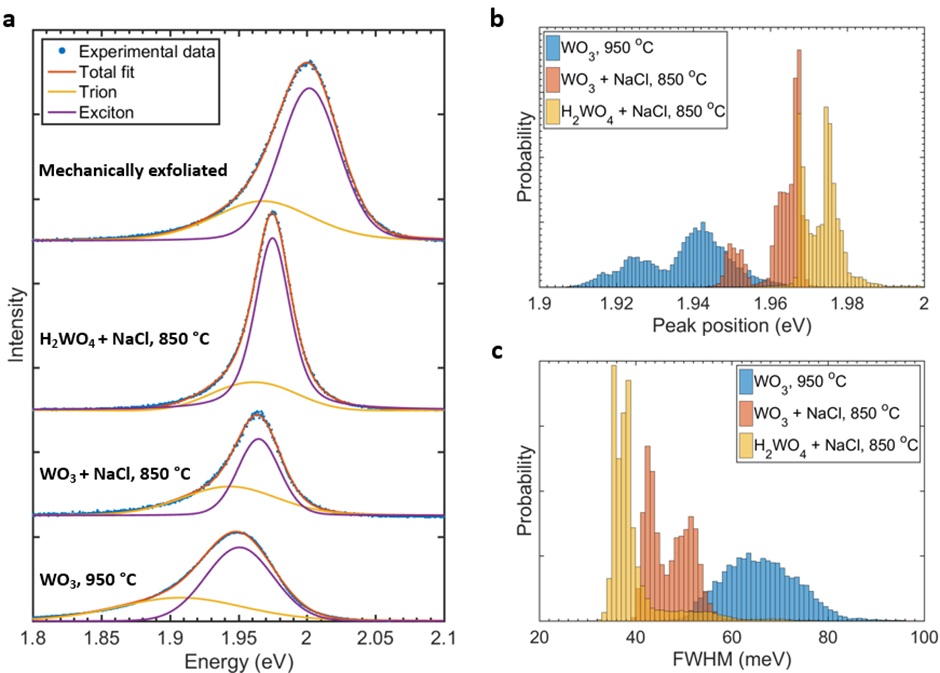
\includegraphics[scale=0.3]{PaperPLSpectraHistograms.png}
\caption{PL spectra characteristics of $WS_2$ grown using: $WO_3$ at 950 {\degree}C, $WO_3+NaCl$ at 850 {\degree}C, $H_2WO_4+NaCl$ at 850 {\degree}C: (a) individual spectra (dotted line) and deconvolution in exciton and trion components; (b) distribution of PL peak position and (c) distribution of PL FWHM for several $WS_2$ grown using the three different precursor systems.}
\label{fig:PaperPLSpectraHistograms}
\end{center}
\end{figure}

As seen in Figure \ref{fig:PaperSIMapsRaman} the Raman peaks are generally uniform in both intensity and position for most samples. The irregularities in the intensity and position of both the $E^1_{2g}$ and $A_{1g}$ in the sample grown at 950 {\degree}C with both $WO_3 + NaCl$ and $H_2WO_4 + NaCl$ are caused primarily by residue deposited on top of the flakes after the growth as seen in optical micrographs. Additionally as seen in Figure \ref{fig:PaperSIMapsIntensityE} the deviations from the mean value are located primarily at the edges of the sample. This suggests that the rest of flake is pristine and the deviations are associated with residue located at the edges. The coefficient of variation (CV) for the intensity and position for the samples grown at 950 {\degree}C with $WO_3$ and at 850 {\degree}C with $WO_3 + NaCl$ and $H_2WO_4 + NaCl$ is on the order of up to $10^{-4}$ which indicates a very high homogenity across the samples. This further shows that the crystal quality of the flakes is quite uniform regardless of the growth method.

\begin{figure}[h]
	\begin{center}
		\begin{subfigure}[b]{0.4\textwidth}
			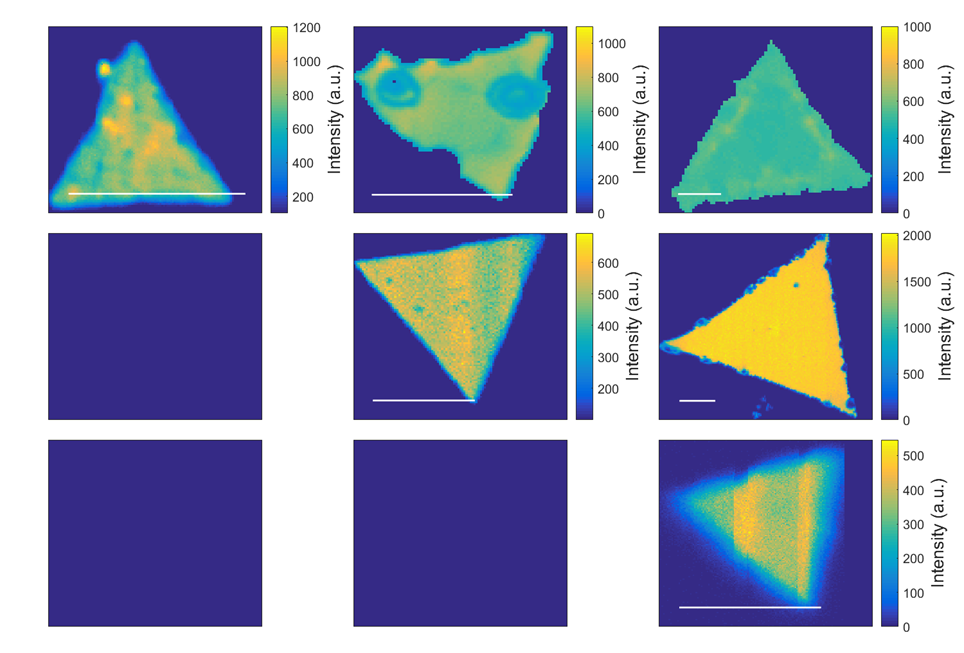
\includegraphics[width=\textwidth]{PaperSIMapsIntensityE.png}
			\caption{Maps of Raman $E^1_{2g}$ peak intensity}
			\label{fig:PaperSIMapsIntensityE}
		\end{subfigure}
		\quad
		\begin{subfigure}[b]{0.4\textwidth}
			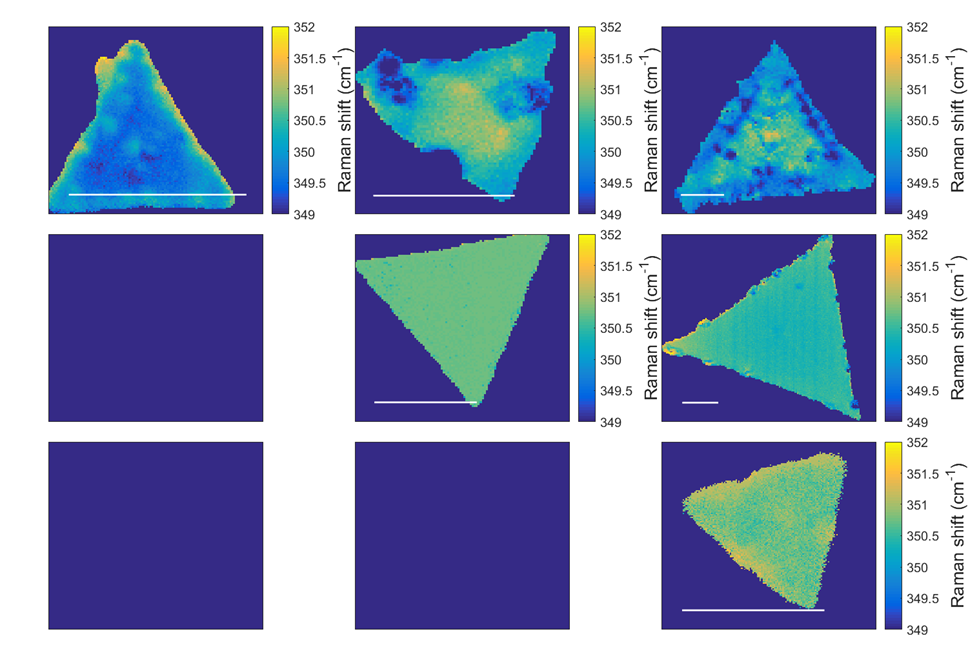
\includegraphics[width=\textwidth]{PaperSIMapsPositionE.png}
			\caption{Maps of Raman $E^1_{2g}$ peak position}
			\label{fig:PaperSIMapsPositionE}
		\end{subfigure}
		\hfill
		\begin{subfigure}[b]{0.4\textwidth}
			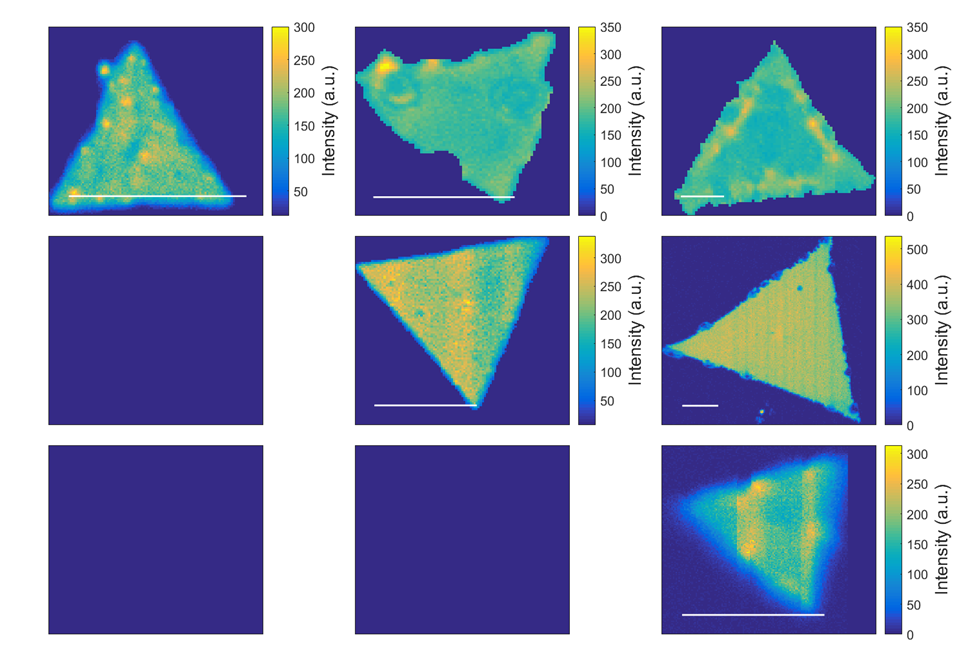
\includegraphics[width=\textwidth]{PaperSIMapsIntensityA.png}
			\caption{Maps of Raman $A_{1g}$ peak intensity}
			\label{fig:PaperSIMapsIntensityA}
		\end{subfigure}
		\quad
		\begin{subfigure}[b]{0.4\textwidth}
			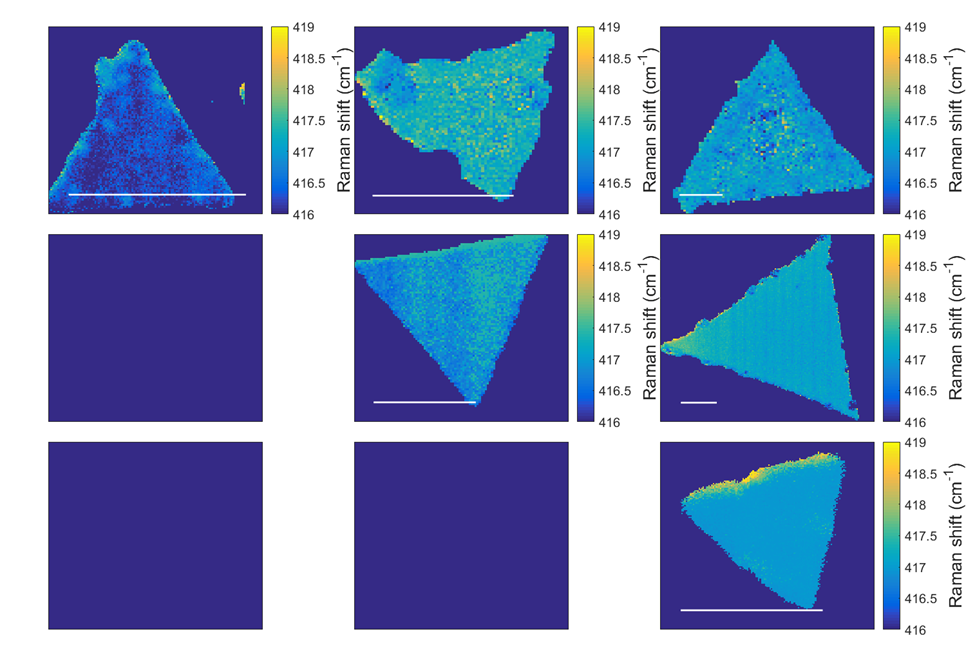
\includegraphics[width=\textwidth]{PaperSIMapsPositionA.png}
			\caption{Maps of Raman $A_{1g}$ peak position}
			\label{fig:PaperSIMapsPositionA}
		\end{subfigure}
		\caption{Maps of Raman peaks intensities and positions}
		\label{fig:PaperSIMapsRaman}
	\end{center}
\end{figure}

By looking at the difference in position between $A_{1g}$ and $E^1_{2g}$ peak positions as seen in Figure \ref{fig:PaperSIMapsDifference} is can be further concluded that the flakes are uniformly monolayer. The deviations from the mean are heavily localised and correlated with differences in PL as well as optical images and are most likely caused by precursors residue. Additionally no trisecting lines (as seen in Figure \ref{fig:PaperPLMaps}) can be seen in the maps of Raman spectra.

\begin{figure}[h]
	\begin{center}
		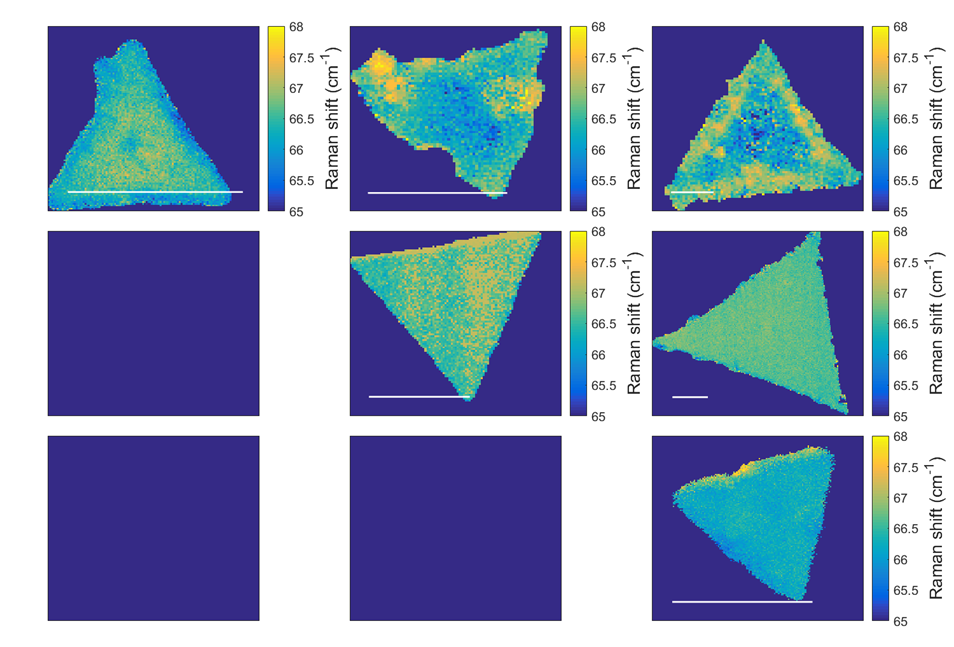
\includegraphics[scale=0.3]{PaperSIMapsDifference.png}
		\caption{Raman spectroscopy: $2LA-A_{1g}$ energy differences. Scale bar is 10 $\mu$m}
		\label{fig:PaperSIMapsDifference}
	\end{center}
\end{figure}

The maps of PL peak positions and widths can be seen in Figure \ref{fig:PaperSIMapsPL}. The PL positions map of the sample grown at 950 {\degree}C using $WO_3$ shows some variability with spots of lower energy that loosely correlate with the PL intensity. There is still faintly visible pattern of three trisecting lines of higher energy as seen in Figure \ref{fig:PaperPLMaps}. This indicates the areas with higher intensity correlate with lower peak position, especially along the trisecting lines. The other maps, especially the ones grown at 850 {\degree}C and 750 {\degree}C with $WO_3 + NaCl$ and $H_2WO_4 + NaCl$, are more uniform in terms of PL peak position and PL peak width. The deviations are again highly localised and correlated with the deviations in Raman and PL intensity. These deviations are generally of lower PL peak position as well as greater PL peak width which generally indicates lower crystal quality.

\begin{figure}[h]
	\begin{center}
		\begin{subfigure}[b]{0.4\textwidth}
			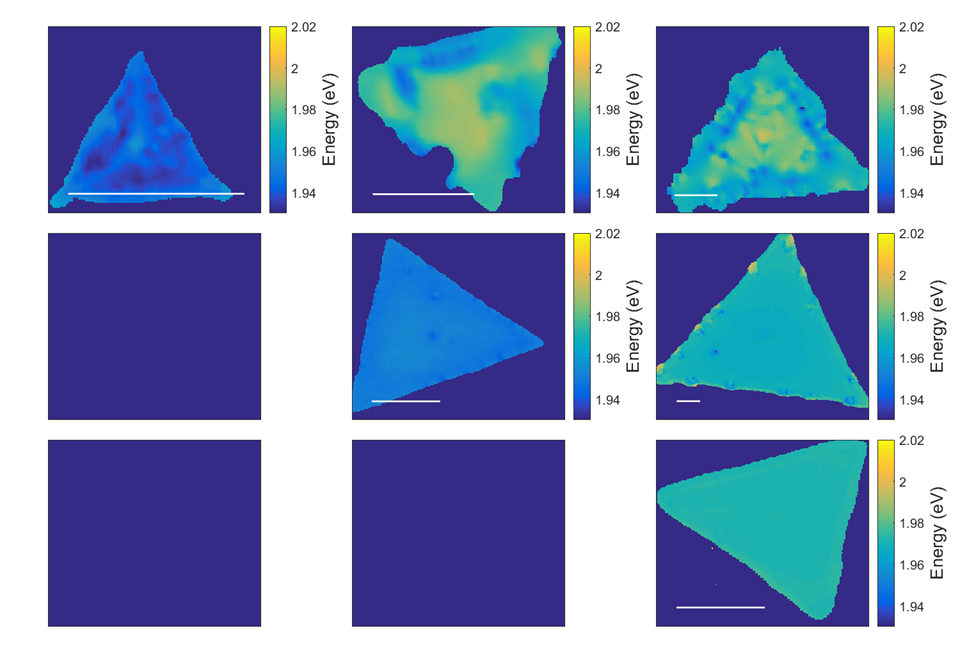
\includegraphics[width=\textwidth]{PaperSIMapsPositionPL.png}
			\caption{Maps of PL peak position}
			\label{fig:PaperSIMapsPositionPL}
		\end{subfigure}
		\quad
		\begin{subfigure}[b]{0.4\textwidth}
			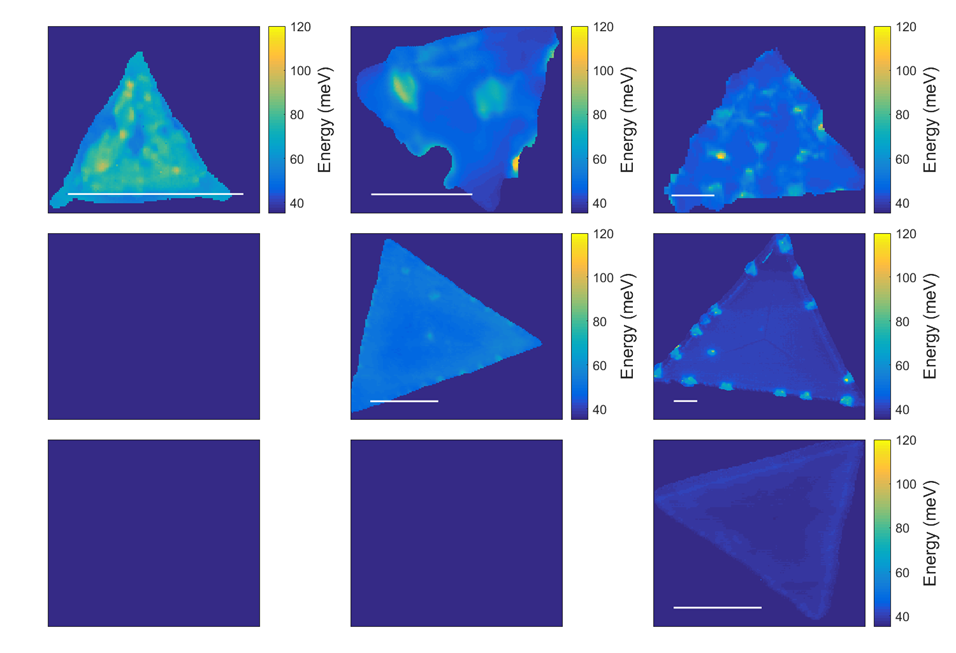
\includegraphics[width=\textwidth]{PaperSIMapsWidthPL.png}
			\caption{Maps of PL peak width}
			\label{fig:PaperSIMapsWidthPL}
		\end{subfigure}
		\caption{Maps of PL peak positions and width}
		\label{fig:PaperSIMapsPL}
	\end{center}
\end{figure}

One possible explanation of the pattern of trisecting lines as seen in e.g. Figure \ref{fig:PaperPLMaps} is the thermal strain caused by difference in thermal expansion coefficient between $WS_2$ and the $SiO_2$ substrate. Since it is known that the strain in TMDCs including $WS_2$ can casue the change in Raman and PL spectrum \cite{Liu2014}\cite{Hui2013} then removing a piece of the material should cause the strain to adapt to new bounding conditions. In order to investigate the trisecting pattern a flake with such pattern has been cut using 532 nm high intensity laser (50 mW). As seen in Figure \ref{fig:PaperSIMapsCutting} both the PL intensity maps and Raman $E^1_{2g}$ maps show a clear separation. The resulting PL and Raman intensity maps however do not show any significant change in the pattern. The trisecting lines as well as local maxima can still be seen in PL intensity map. The Raman shows few spots of increased intensity on of the halves of the flake as well as a very weak increased intensity area along the cut. Since there is no observed increased intensity along any edges before cutting the flake it does not appear that the increased intensity along the cut is a result of strain being resolved into new bounding conditions. It appears therefore that cutting the material did not alter the pattern nor alter the rest of the PL or Raman spectra maps.

\begin{figure}[h]
	\begin{center}
		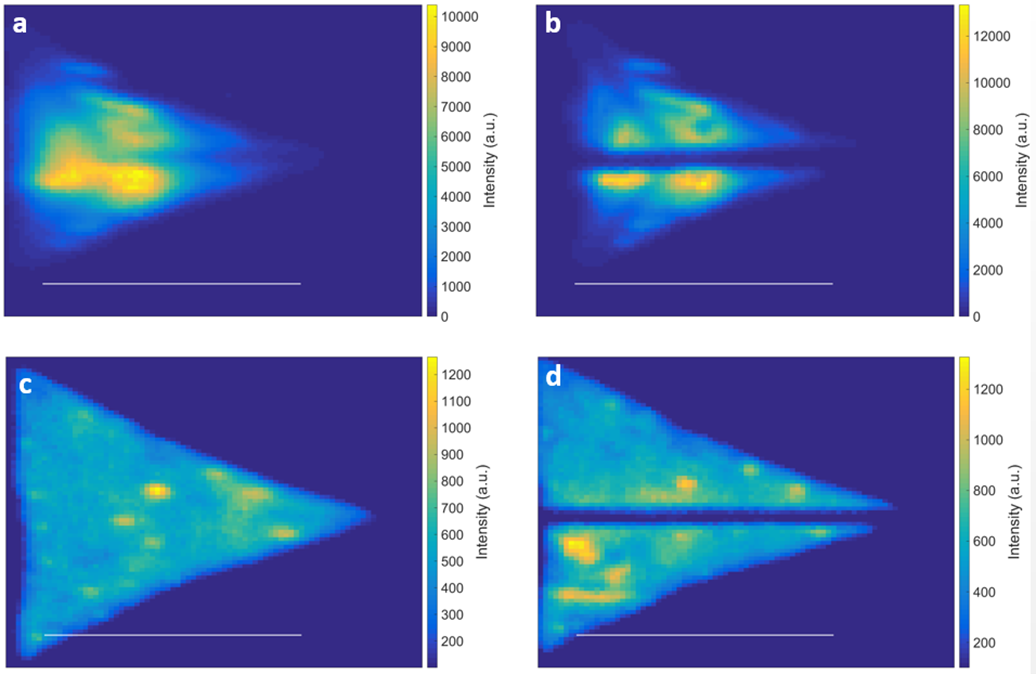
\includegraphics[scale=0.3]{PaperSIMapsCutting.png}
		\caption{PL intensity (a) before and (b) after the cutting. $2LA+E^1_{2g}$ Raman intensity (c) before and (d) after the cutting. Scale bar is 10 $\mu$m}
		\label{fig:PaperSIMapsCutting}
	\end{center}
\end{figure}

The spectral maps from different flakes grown with the same conditions were then collected and plotted as graphs of intensity or width versus position. As seen in Figure \ref{fig:PaperSIScatterComparison} the PL intensity seems to be largely independent of the PL position. If PL is present at given position then intensity is mostly uniformly distributed in terms of intensity. The PL width seems to be inversely related with regards to PL position. In samples grown at 850 {\degree}C with $WO_3 + NaCl$ the relation seems to be the strongest. Across all the samples the values vary between around 60-80 meV at low PL energies (1.92 eV) to 40-60 meV at high PL energies (1.98 eV). This seems to be related to overall quality of the crystals, i.e. the presence of defects, stoichiometry, crystallinity, doping, adatoms. The more uniform the sample the less mechanisms for peak broadening as well as fewer added energy levels facilitating different electron recombination paths.

\begin{figure}[!h]
	\begin{center}
		\begin{subfigure}[b]{0.8\textwidth}
			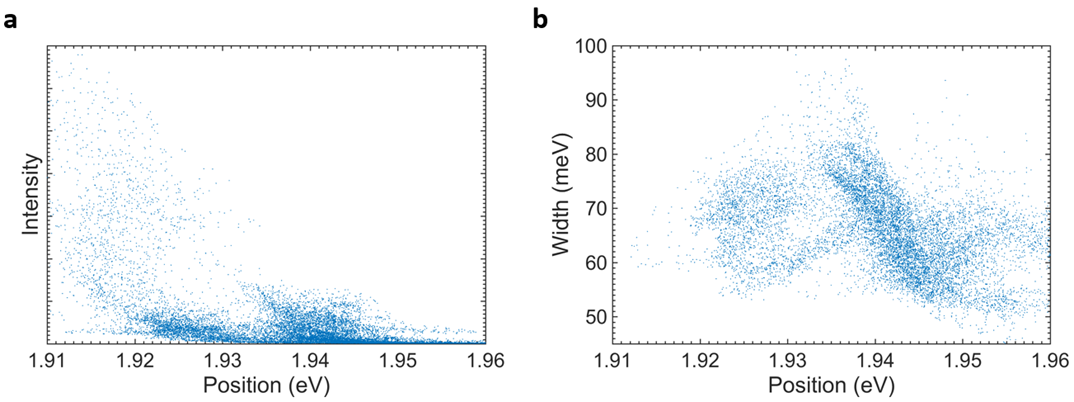
\includegraphics[scale=0.3]{PaperSIScatterWO3.png}
			\caption{(a) PL Intensity vs position, (b) PL FWHM vs position of $WS_2$ grown using $WO_3$ at 950 {\degree}C}
			\label{fig:PaperSIScatterWO3}
		\end{subfigure}

		\begin{subfigure}[b]{0.8\textwidth}
			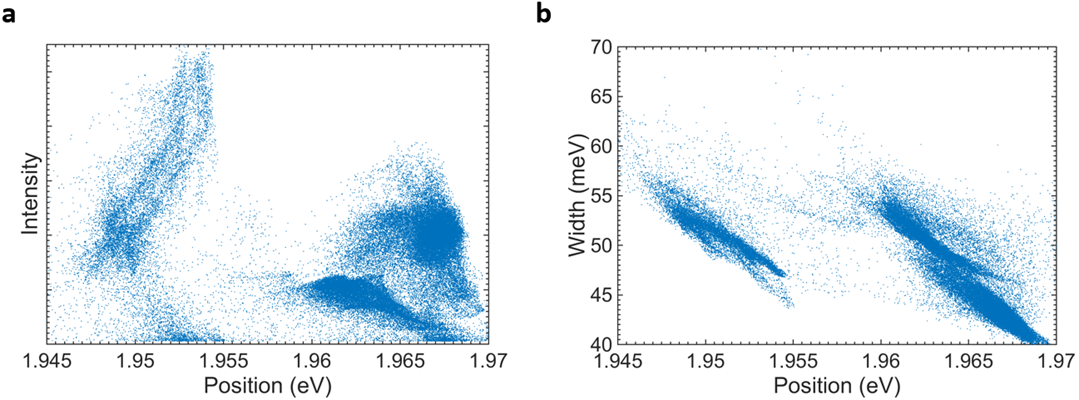
\includegraphics[scale=0.3]{PaperSIScatterWO3NaCl.png}
			\caption{PL Intensity vs position, (b) PL FWHM vs position of $WS_2$ grown using $WO_3+NaCl$ at 850 {\degree}C}
			\label{fig:PaperSIScatterWO3NaCl}
		\end{subfigure}

		\begin{subfigure}[b]{0.8\textwidth}
			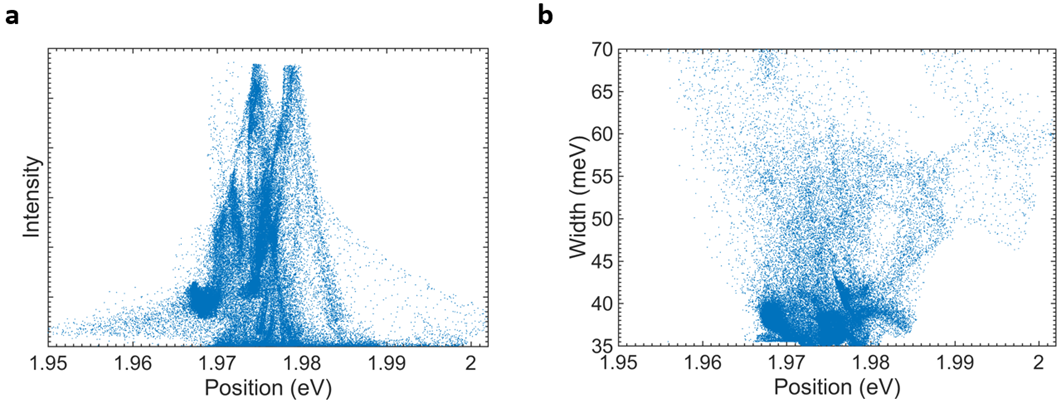
\includegraphics[scale=0.3]{PaperSIScatterH2WO4NaCl.png}
			\caption{(a) PL Intensity vs position, (b) PL FWHM vs position of $WS_2$ grown using $H_2WO_4+NaCl$ at 850 {\degree}C}
			\label{fig:PaperSIScatterH2WO4NaCl}
		\end{subfigure}

		\begin{subfigure}[b]{0.8\textwidth}
			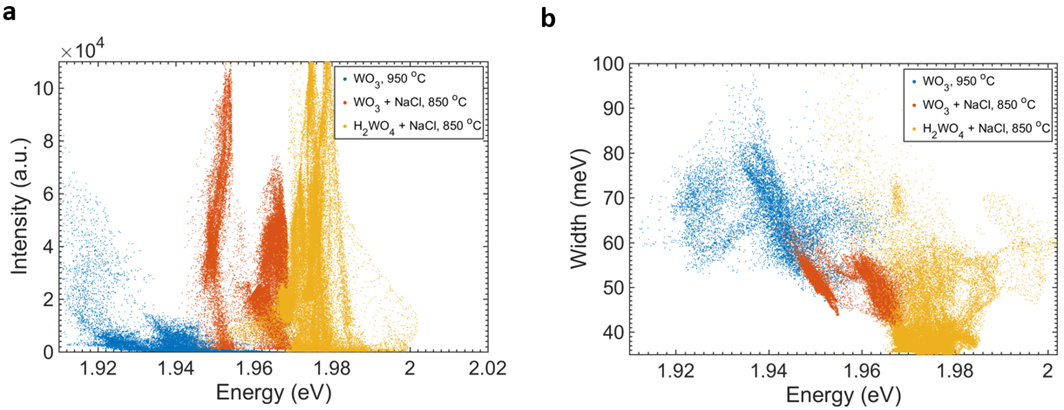
\includegraphics[scale=0.3]{PaperSIScatterComparison.png}
			\caption{(a) PL Intensity vs position, (b) PL FWHM vs position of $WS_2$ grown using $WO_3$, $WO_3+NaCl$, $H_2WO_4+NaCl$}
			\label{fig:PaperSIScatterComparison}
		\end{subfigure}
	\end{center}
\end{figure}

The chemical composition of the flakes grown using $H_2WO_4 + NaCl$ has been investigated using XPS. The W 4f5/2 and W 4f7/2 core levels show peak positions that of the $W^{4+}$ in $WS_2$ \cite{Cattelan2015}\cite{Martinez2004} (32.7 eV 34.8 eV respectively) with FWHM of 1 eV (Figure \ref{fig:PaperXPS}, the smallest possible using Mg K$\alpha$ x-ray source. It means therefore that the $WS_2$ is of perfect stoichiometric ratio of W and S. Additionally by integrating the intensity of the W 4f and S 2p core level peaks the same result is achieved. Furthermore the S 2p1/2 and 2p3/2 core levels are also present at the expected position for $WS_2$ (162.3 eV and 163.4 eV respectively, Figure \ref{fig:PaperXPS}) and small FWHM of 1 eV \cite{Martinez2004}. Small peaks indicative of $W^{6+}$ (W 4f5/2 and W 4f7/2 at 35.9 eV and 38.1 eV respectively, Figure \ref{fig:PaperXPS}) can be attributed to presence of $WO_3$ and which partially overlaps with W 5p core level (38.5 eV). These peaks however disappear after the flakes are transferred to another $Si/SiO_2$ substrate, suggesting that they can be caused by residue $WO_3$ given that the XPS spot size is relatively big ({$\sim$}1 mm). The FWHM of the W 4f core levels was unchanged after the transfer, indicating that the crystallinity and the quality of the flakes was preserved with no extra defects introduced.

The $WS_2$ samples grown using $WO_3 + NaCl$ have been characterised by XPS as well and the stoichiometric ratio of 2:1 for S:W has been found. However the $W^{6+}$ component, caused most likely by presence of $WO_3$ (W 4f5/2 and W 4f7/2 at 35.9 eV and 38.1 eV respectively) is more pronounced indicating incomplete sulfurisation. Similarly to the sample grown with $H_2WO_4 + NaCl$ this component disappears entirely upon transferring the sample onto new $Si/SiO_2$ indicating it is present around the flakes, distributed across the substrate. The $W^{4+}$ 4f core levels peak width is {$\sim$}1.2 eV which indicates higher defect concentration compared to that of the sample grown using $H_2WO_4 + NaCl$. This FWHM however increases after the transfer, which is most likely caused by the increase in the concentration of the defects caused by the mechanical stress during the transfer. In conclusion the $H_2WO_4$ is shown to be a better precursor compared to $WO_3$.
 
\begin{figure}[h]
\begin{center}
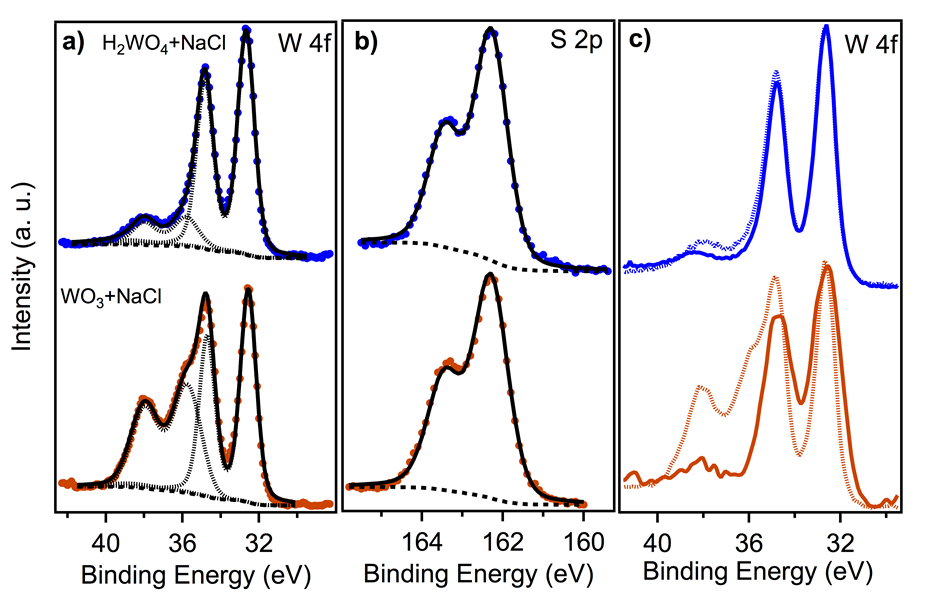
\includegraphics[scale=0.3]{PaperXPS.png}
\caption{XPS spectra of the W 4f and S 2p core level peak regions. (a) Comparison  of W 4f5/2 , W 4f7/2  and W 5p core levels of WS2 grown using H2WO4+NaCl at 950 {\degree}C (blue spectrum) with WS2 grown using WO3+NaCl at 950 {\degree}C (red spectrum). The deconvolution of W 4f5/2 , W 4f7/2  and W 5p core levels and overall fit of the spectrum are reported as black dashed and a continuous line respectively. (b) The S 2p1/2 and 2p3/2 core levels for each of the two growth conditions are reported in the central panel. (c) W 4f5/2 , W 4f7/2  and W 5p core levels before (dashed line) and after transfer (continuous like) onto a new SiO2/Si substrate are compared showing the complete disappearance of the residual WO3 components. The spectra were fit by Doniach-Sunjic function after subtracting a Shirley background (black dashed line).}
\label{fig:PaperXPS}
\end{center}
\end{figure}

The samples were further characterised for their electrical properties. Bottom-gated field effect transistors were prepared as seen in Figure \ref{fig:PaperElectricalMeasurementMonolayer}. The FET transfer curve indicates accumulation-type n-channel transistor, where the drain current increases with applied gate bias after a threshold is crossed. Once the current-bias curve reaches linear range it can be described by $I_d = {\mu}_nC_{ox}(W/L) ((V_{gs}-V_{th})V_{ds})$, where ${\mu}_n$ is the electron field-effect mobility, $C_ox$ is the oxide dielectric and $V_th$ is the threshold voltage. As seen in Figure \ref{fig:PaperElectricalMeasurementMonolayer} a typical response curve for both the as grown as well as transferred samples of $WS_2$ grown with $H_2WO_4$ show an asymmetry around $V_{ds}=0$ V due to difference in the source and drain potentials. The Schottky barrier at the source is pinned by the gate, while the barrier at the drain diminishes proportionally to the drain bias and vice versa. The contacts however become more "Ohmic", when the bands bend more at the semiconductor/metal interface while the gate bias increase, leading to more significant tunnelling current.

\begin{figure}[h]
\begin{center}
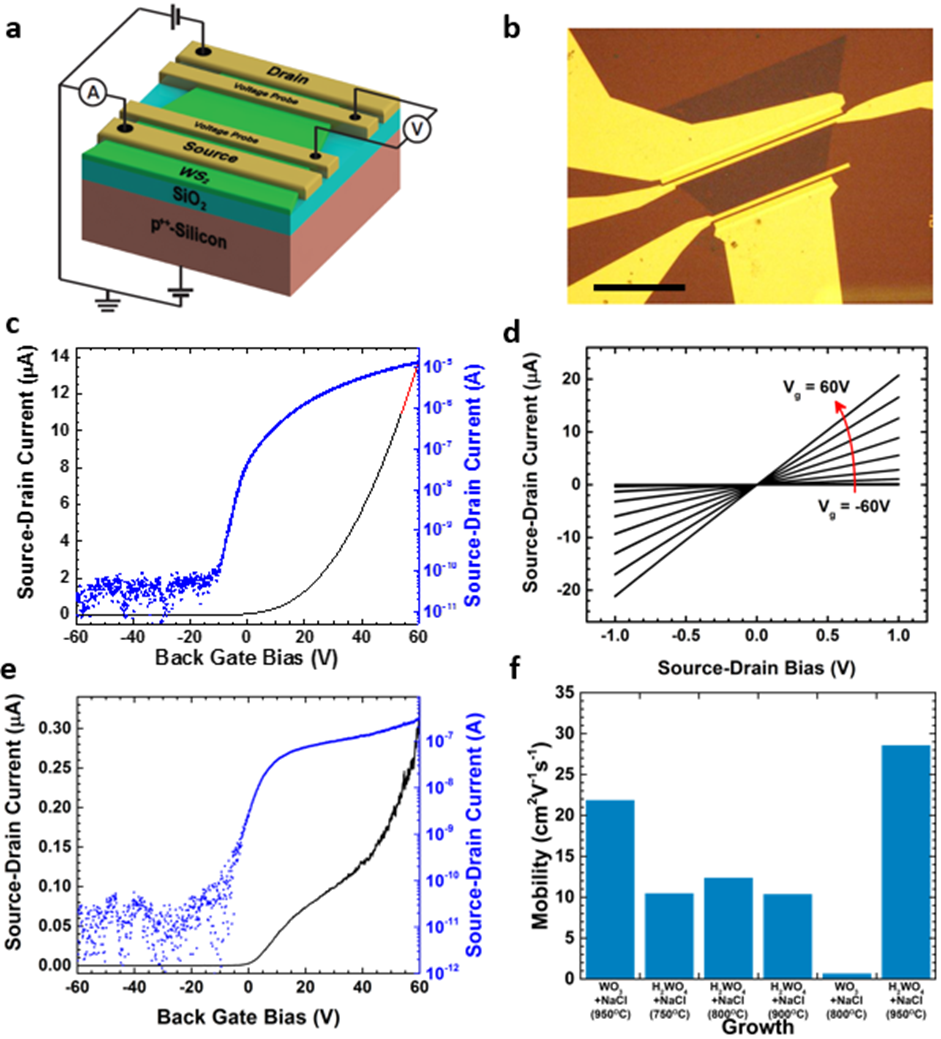
\includegraphics[scale=0.3]{PaperElectricalMeasurementMonolayer.png}
\caption{Electrical characteristics of monolayer WS2: (a) Schematic of the bottom-gated field effect transistors; (b) optical micrograph of the device (scale bar is 20${\mu}$m); (c) FET transfer curve for the monolayer WS2 grown using H2WO4+NaCl at 950 {\degree}C showing the highest mobility of 28 cm2/Vs (linear region of the transport graph marked with a red-dashed line); (d) Response curves at different gate biases for a WS2 triangle grown using H2WO4+NaCl; (e) FET transfer curve for the monolayer WS2 grown using WO3+NaCl at 800 {\degree}C; (f) electron mobilities of monolayer WS2 grown using different conditions.}
\label{fig:PaperElectricalMeasurementMonolayer}
\end{center}
\end{figure}

By looking at the linear regime of the transport graph (red-dashed line in Figure \ref{fig:PaperElectricalMeasurementMonolayer}) the field-effect mobility can be calculated as ${\mu}_n=C_{ox}^{-1}(d{\sigma}/dV_{gs})$. The electron mobility calculated for $WS_2$ grown with $H_2WO_4 + NaCl$ is generally higher than that of $WS_2$ grown with $WO_3 + NaCl$ (Figure \ref{fig:PaperElectricalMeasurementMonolayer}) which further indicates higher crystal quality when using $H_2WO_4$. The monolayer $WS_2$ exhibits electron mobility of 28 $cm^2 V^{-1} s^{-1}$, the highest reported value for CVD grown $WS_2$ and transferred onto $SiO_2$ \cite{Li2015}\cite{Kang2015}\cite{Gao2015}\cite{doi:10.1021/nn403454e}\cite{doi:10.1021/acsnano.5b01480}\cite{Lee2013}\cite{Yun2015}\cite{Alharbi2016}\cite{Lan2015}\cite{Hussain2013}\cite{Cui2015} and comparable to mechanically exfoliated $WS_2$ \cite{Withers2014}\cite{Iqbal2016}\cite{Georgiou2014}\cite{Iqbal2015a}. The highest mobilities were recorded in $WS_2$ grown at 950 {\degree}C, grown with either $H_2WO_4 + NaCl$ or $WO_3 + NaCl$, which indicates a role of the growth temperature in improving the quality of the $WS_2$. As the temperature is lowered the difference between precursors becomes more pronounced in terms of the crystal quality. The $H_2WO_4 + NaCl$ precursor system grown $WS_2$ shows electron mobility of 10 to 20 $cm^2 V^{-1} s^{-1}$ at temperatures of 750 {\degree}C and 850 {\degree}C. The electron mobilities of $WS_2$ grown using $WO_3 + NaCl$ are much lower, {$\sim$}2 $cm^2 V^{-1} s^{-1}$ at 800 $\sim$C. Bilayer $WS_2$ samples have overall greater electron mobility than their monolayer equivalent (between {$\sim$}38 $cm^2 V^{-1} s^{-1}$ and 52 $cm^2 V^{-1} s^{-1}$), similarly to the mechanically exfoliated flakes \cite{Ovchinnikov2014}\cite{Iqbal2015a}. The electron mobility of bilayer $WS_2$ (52 $cm^2 V^{-1} s^{-1}$) (Figure \ref{fig:PaperElectricalMeasurementBilayer} and Figure \ref{fig:PaperMobilityComparison}) is also higher than that of other CVD grown $WS_2$ as well as mechanically exfoliated onto $SiO_2$ samples of $WS_2$ reported  \cite{Iqbal2015}\cite{Ovchinnikov2014}\cite{Iqbal2015a}. The highest mobility has been obtained for bilayer system using $WO_3 + NaCl$ indicating that the precursor choice is less important for electron mobility in such systems. 

\begin{figure}[h]
\begin{center}
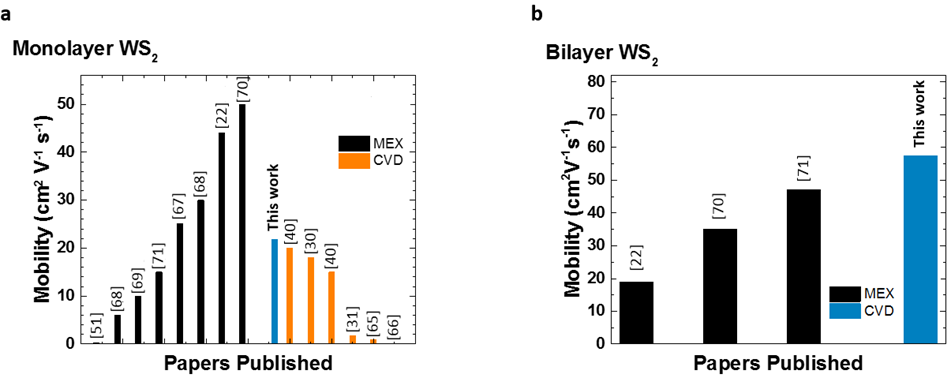
\includegraphics[scale=0.3]{PaperMobilityComparison.png}
\caption{Comparison of our results with the literature of CVD grown material and mechanically exfoliated WS2 (MEX) : electron mobility for (a) monolayer WS2 and (b) bilayer WS2. The histograms show our record values for both monolayer and bilayer amongst the best values reported for CVD grown WS2.}
\label{fig:PaperMobilityComparison}
\end{center}
\end{figure}
 
\begin{figure}[h]
\begin{center}
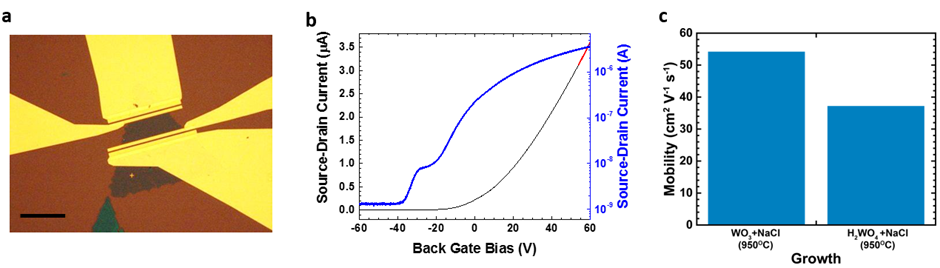
\includegraphics[scale=0.3]{PaperElectricalMeasurementBilayer.png}
\caption{Electrical characteristics of bilayer WS2: (a) Optical micrograph of the device (scale bar is 30$\mu$m); (b) FET transfer curve for the bilayer WS2 grown using WO3+NaCl at 950 {\degree}C showing the highest mobility of 52 cm2/Vs (linear region of the transport graph marked with a red-dashed line); (c) electron mobility of bilayer WS2 grown by using different precursor systems.}
\label{fig:PaperElectricalMeasurementBilayer}
\end{center}
\end{figure}

\section{Conclusions}

In conclusion a synthesis route has been developed that allows for high quality monolayer and bilayer $WS_2$ CVD growth. This quality is demonstrated by highest recorded electron FET mobility for both monolayer and bilayer CVD grown $WS_2$ compared to the literature and comparable to that of mechanically exfoliated ones. Additionally the triangle flakes grown using $H_2WO_4 + NaCl$ are much larger (up to {$\sim$200-300 $\mu m$) compared to ones grown using standard $WO_3$. The CVD growth using $H_2WO_4$ has also been demonstrated to work at lower temperatures, down to 750 {\degree}C compared to more commonly used 950 {\degree}C. Finally the PL of the $WS_2$ grown using $H_2WO_4$ is is uniform throughout the flake and has very FWHM (36 meV) which again points to high crystal quality and lack of defects in form of sulfur vacancies. These findings allow to develop further the TMDCs synthesis method of CVD and can potentially lead to industrially scalable synthesis of monolayer $WS_2$ or other TMDCs over large area.